% Generated by tools/make_figures.py. Needs \usetikzlibrary{positioning}.
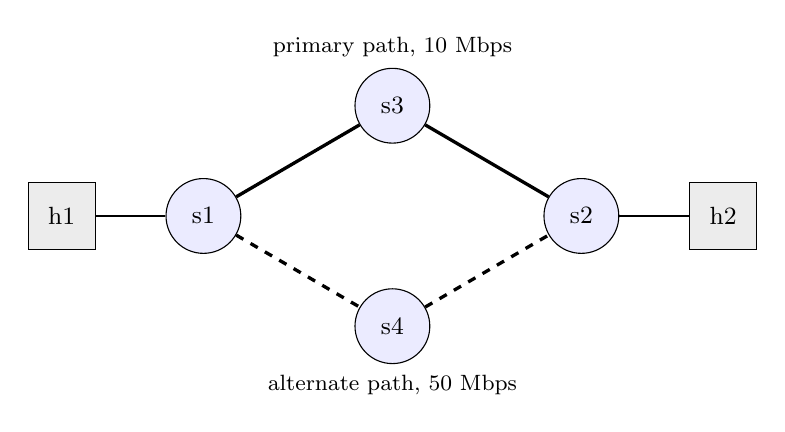
\begin{tikzpicture}[
    sw/.style={draw, circle, fill=blue!8, minimum size=0.95cm, font=\small},
    host/.style={draw, rectangle, fill=gray!15, minimum size=0.85cm, font=\small}]
  \node[host] (h1) at (0,0) {h1};
  \node[sw] (s1) at (1.8,0) {s1};
  \node[sw] (s3) at (4.2,1.4) {s3};
  \node[sw] (s4) at (4.2,-1.4) {s4};
  \node[sw] (s2) at (6.6,0) {s2};
  \node[host] (h2) at (8.4,0) {h2};
  \draw (h1) -- (s1);
  \draw (s2) -- (h2);
  \draw[very thick] (s1) -- (s3) -- (s2);
  \draw[very thick, dashed] (s1) -- (s4) -- (s2);
  \node[font=\footnotesize, above] at (4.2,1.9) {primary path, 10 Mbps};
  \node[font=\footnotesize, below] at (4.2,-1.9) {alternate path, 50 Mbps};
\end{tikzpicture}
